\documentclass[a4paper]{article}


%%% ENCODING, FONT & LOCALIZATION
\usepackage[utf8]{inputenc} % use unicode input-encoding (allows unicode characters in the .tex files, default: Asci)
\usepackage{lmodern} % vectorized version of the "computer modern" font (default) (https://tex.stackexchange.com/q/1390/148164, https://tex.stackexchange.com/q/147194/148164)
\usepackage[ngerman, english]{babel} %% last language is main
%\shorthandoff{"} %babel breaks tikz-cd otherwise (activate if used)
\usepackage{csquotes} %% biblatex wants csquotes (localized quotes) if babel is present

%%% GENERAL IMPROVEMENTS
\usepackage[unicode, hidelinks]{hyperref} %% clickable links
\usepackage{enumitem} %% better (customizable) enumerations (e.g. \begin{enumerate}[label=(\roman*)])


%%% STYLING
% \setlength{\parindent}{0em} % No indentation for new paragraphs
\usepackage{emptypage} % removes page numbers on empty pages
% \makeatletter \@twosidefalse \makeatother
\usepackage{xcolor}


%%% GRAPHICS & PLOTS

% \usepackage{graphicx} % enable pictures
\usepackage{wrapfig} % text wrapping around figures
% \usepackage{tikz, tikz-cd, pgfplots} % plots and sketches
% \pgfplotsset{compat=1.16}

%%% CODE
\usepackage[ruled,linesnumbered]{algorithm2e}
\usepackage{minted}

% fix algomathdisplay (see: https://tex.stackexchange.com/a/611426/148164)
\makeatletter
\renewenvironment{algomathdisplay}
 {\[}
 {\@endalgocfline\vspace{-\baselineskip}\]{\DontPrintSemicolon\;}}
\makeatother
%%% MATH
\usepackage{mathtools} % fixes some things from amsmath and adds some new features
\usepackage{amsthm, amssymb} % amsthm -> proof env, amssymb -> additional symbols
\usepackage{aligned-overset} % https://tex.stackexchange.com/questions/257529/overset-and-align-environment-how-to-get-correct-alignment
%% usage: \overset{something}&{=}

%%% Special Symbols
% \usepackage{bbm} % blackboard numbers: usage \mathbbm{1} (amssymb \mathbb{1} looks bad)
% \usepackage{cancel} % strike through equation parts to indicate they cancel out
% %% contradiction symbol
% \usepackage{wasysym} % lightning symbol
% \newcommand*{\contradiction}[1][]{\quad\text{{\LARGE\lightning} #1}\ }

%%% EDITING (Annotations, TODO, etc.) 
\usepackage[draft]{fixme} %final removes annotations %draft includes annotations
\fxsetup{theme=color}
%%\fxnote{some note} ,\fxwarning{}, \fxerror{}, \fxfatal{} <- does not allow [final] to compile

%%% BIBLIOGRAPHY
\usepackage[style=alphabetic, backend=biber, seconds=true, date=iso, urldate=iso, maxcitenames=2]{biblatex}
\addbibresource{references.bib}

%% AMS Theorem Environments
\theoremstyle{plain}% default
\newtheorem{prop}{Proposition}[section]
\newtheorem{lemma}[prop]{Lemma}
\newtheorem{corollary}[prop]{Corollary}
\newtheorem{theorem}[prop]{Theorem}

\theoremstyle{definition}
\newtheorem{definition}[prop]{Definition}
\newtheorem{example}[prop]{Example}
\newtheorem{assumption}[prop]{Assumption}

\theoremstyle{remark}
\newtheorem{remark}[prop]{Remark}

%%

\newcommand{\E}{\mathbb{E}}
\renewcommand{\Pr}{\mathbb{P}}
\DeclareMathOperator{\sgn}{sgn}
\newcommand{\identity}{\mathbb{I}}
\newcommand{\normal}{\mathcal{N}}
\newcommand{\dimension}{d}
\newcommand{\C}{\mathcal{C}}
\DeclareMathOperator{\chol}{chol}


\title{Incremental Gaussian Process}
\author{Felix Benning, Alexander Freudenberg}

\begin{document}
	\maketitle 
	\begin{abstract}
	Lorem Ipsum etc.	
\end{abstract}

	\section{Simulating Gaussian Random Variables}

To simulate \(X_{1:n} = (X_1,\dots,X_n)^T \sim \normal(0, \Sigma_n)\) one typically
searches for \(L_n\) such that
\[
	L_n L_n^T = \Sigma_n,
\]
because for \(Y_{1:n}\sim\normal(0,\identity)\) independent standard normal
random variables we have
\[
	X_{1:n} = L_n Y_{1:n} \sim \normal(0, \Sigma_n).
\]
In particular for a centered gaussian process/random field 
\(Z=(Z(x))_{x\in\real^\dimension}\) with covariance function \(\C\),
we can simulate \((Z(x_1),\dots, Z(x_n))\) by calculating \(\Sigma_n\) from its
covariance function
\[
	\Sigma_n = \begin{pmatrix}
		\C(x_1, x_1) &\dots &\C(x_1, x_n)\\
		\vdots &  & \vdots \\
		\C(x_n, x_1) &\dots &\C(x_n, x_n)
	\end{pmatrix}.
\]
But what if you already have simulated \((Z(x_1),\dots,Z(x_n))\) and now want
to obtain \(Z(x_{n+1})\) without changing your previous values? If you wanted
to do optimization on a random field for example, \(X_{n+1}\) might even be a
random variable depending on the previous results. You can hardly start over
in this case.

The package ``IncrementalGRF.jl'' available on GitHub
\url{https://github.com/FelixBenning/IncrementalGRF.jl} is built with this
Incremental evaluation in mind without sacrificing any performance compared to
batch evaluation.

Its interface is simple

\begin{minted}{julia}
using IncrementalGRF

dim = 2 # input dimension
rf = GaussianRandomField(
	# passing the covariance kernel
	Kernels.SquaredExponential{Float64, dim}(1)
) # rf represents one realization of the entire Gaussian Random Field Z
rf([0., 0]) # rf(0,0) = Z(0,0)(omega)
rf([1., 0]) # rf(1,0)

# the dot notation broadcasts the "function" rf over the input array
# i.e. applies it element-wise resulting in [rf(3,0), rf(0,1)]
rf.([
  [3., 0],
  [0., 1.]
])
\end{minted}
An instance of type ``GaussianRandomField'' therefore represents the realization
of the entire random field \(Z\). As that would be infinite dimensional it can
not actually eagerly determine this entire random field, so it lazily
adds evaluations to its internal state whenever invoked.

It turns out that knowing all the evaluation points beforehand does not actually
help asymptotic performance. In reality there is a slight improvement due to
memory access issues. But if you incrementally provide the next \(k\) points
instead of all points at once where \(k\) is large enough, then there is no
real difference either. This is especially interesting for random fields with
\(k\) output dimensions, because you can rewrite \(Z_i(x)\) into \(Z(x,i)\). So
evaluating \(Z\) at one point requires the evaluation of \(k\) points
\[
	Z(x) = (Z(x,1),\dots,Z(x,k)).
\]
An example for such a use case, is simulation of the gaussian random field
\((Z,\nabla Z)\), which has \(\dimension+1\) out-dimensions for \(\dimension\)
inputs.

\subsection{Caveat: No pivot}

While this method has no drawbacks compared to the standard cholesky
decomposition, it has no analog for the pivoted cholesky decomposition. The
pivoted cholesky decomposition essentially reorders the evaluation points for
numerical stability. And since we are incrementally evaluating our random field,
we can not retroactively change the order of evaluation.


	\section{Incremental Cholesky}

Assuming we already have the cholesky decomposition \(L_n\) of \(\Sigma_n\),
can we find the cholesky decomposition \(L_{n+1}\) of the extended covariance
matrix \(\Sigma_{n+1}\) faster? It turns out yes, as
\[
	\begin{aligned}
	L_{n+1}L_{n+1}^T
	&=\begin{pmatrix}
		L & \\
		l^T &\lambda
	\end{pmatrix}
	\begin{pmatrix}
		L^T &  l\\
		&\lambda^T
	\end{pmatrix}
	= \begin{pmatrix}
		L L^T & L l\\
		l^T L^T & l^T l + \lambda\lambda^T
	\end{pmatrix}\\
	\overset!&= \begin{pmatrix}
		\Sigma_n & c_n \\
		c_n & \sigma_n^2
	\end{pmatrix} = \Sigma_{n+1}
	\end{aligned}
\]
implies \(L = L_n\) and
\[
	l_n := l = L^{-1}c_n.
\]
And finally
\[
	\lambda_n := \lambda = \sqrt{\sigma_n^2 - l^T l}.
\]

If we now apply \(L_{n+1}\) to \(Y_{1:(n+1)}\), we get
\[
	Z_{1:(n+1)}
	= \begin{pmatrix}
		L_n & \\
		l_n^T & \lambda_n
	\end{pmatrix}
	Y_{1:(n+1)}
	= \begin{pmatrix}
		L_n Y_{1:n} \\
	 	l_n^T Y_{1:n} + \lambda_n Y_{n+1}
	\end{pmatrix}
\]
So if we reuse \(Y_{1:n}\), then we will also get the same \(Z_{1:n}\). Assuming
\(L_n\) is invertible (\(\Sigma_n\) strictly positive definite), we have
\[
	\E[Z_{n+1}\mid Z_{1:n}]
	= \E[Z_{n+1}\mid Y_{1:n}] = \langle l_n, Y_{1:n}\rangle.
\]
So \(\lambda_n\) represents the conditional standard deviation, \(Y_{n+1}\) the
``new randomness''.

If we have already returned \(Z_{1:n}\) previously, we only need to
\begin{enumerate}
	\item Generate a new independent standard Gaussian random variable \(Y_{n+1}\)
	\item Calculate \(l_n = L_n^{-1}c_n\) and \(\lambda_n = \sqrt{\sigma_n^2- l_n^T l_n}\)
	\item Return \(Z_{n+1} = \langle l_n, Y_{1:n}\rangle + \lambda_n Y_{n+1}\)
\end{enumerate}
We only need to store \(L_n\) and \(Y_{1:n}\). In the case of random fields,
it is typically also necessary to store the points \((x_1,\dots, x_n)\), where
the random field was evaluated so far. Because we need them to calculate the
covariance \(c_n\) with a new point.


\subsection{Performance}

It turns out, that adding the row \((l_n^T ,\lambda_n)\) to \(L_n\) is exactly
how the Cholesky-Banachiewicz algorithm for determining the Cholesky
decomposition is defined. So we are literally doing the exact same calculations.
The only change is the order of the operations. So the question is how memory
access friendly the respective algorithms are. The advantage is, that we do not
have to fetch all the rows from memory once we want to multiply
\(L_n\) with \(Y_{1:n}\). Instead we can do this multiplication immediately after
we calculated \(l_n\) and \(\lambda_n\). But we do have to repeatedly retrieve
\(Y_{1:n}\) on the other hand. So in this sense the effect cancels out.

To store the \(Y_{1:n}\) we simply use a dynamic array. To save the matrix \(L_n\)
we do not want to use a normal \(2\) dimensional array. Because, to extend a
matrix by one row and column, you would have to extend the rows by one, which
are stored one after the other in a row major format which essentially
requires moving all of them (analogously columns in column major).

So instead we want to use packed storage
\[
	\begin{bmatrix}
		L_{11}	
	\end{bmatrix}
	\begin{bmatrix}
		L_{21} & L_{22}
	\end{bmatrix}
	\begin{bmatrix}
		L_{31} & L_{32} & L_{33}
	\end{bmatrix}
	\dots
\]
As we only need to append \((l_n^T, \lambda_n)\), we can again use a dynamic
array. Unfortunately packed storage only allows vectorized BLAS routines
(BLAS-2) but not block-wise operations (BLAS-3). And similarly the most performant
cholesky decompositions want to access the data block-wise. So adding just one
row \(l_n^T\) is not as performant as adding a block. To fix the first problem
we propose ``Block Packed Storage'', which we will describe in Section~\ref{sec: memory
layout}. To solve the second problem, one needs to aks for \(k\) new points in
batches as described in the introduction. For random fields with large enough
output dimension, this is not a problem as mentioned. But for the benefit of
random fields with small output dimension, it makes sense to specialize
\begin{minted}{julia}
	Base.broadcasted
\end{minted}
in order for \mintinline{julia}{rf.(all_evaluation_points)} to be as performant
as possible.

Lastly one can improve on the allocation performance of dynamic arrays, by implementing
\begin{minted}{julia}
	sizehint!(::GaussianRandomField, ::Int)	
\end{minted}
by translating the size requirements for the given number of points into a
\mintinline{julia}{sizehint!} for the underlying dynamic arrays. But as
\mintinline{julia}{sizehint!} is just a suggestion but not a guarantee, the
checks at every \mintinline{julia}{push!} have to remain. That
cost is negligible though, in comparison to the cost of calculating the
value of the random field at the point, due to the \(O(n^2)\) complexity of
calculating a single value. But again a specialization of
\mintinline{julia}{Base.broadcasted} can remove even this tiny speed bump.

\subsection{Numerical Stability}

Numerical errors might cause \(\sigma^2 - l^T l\) to be negative which
represents a negative conditional variance. In other words: the existing points
explain the new point so well (\(l^Tl\) is large), such that almost no
randomness is left and numerical errors make the randomness negative. This
happens especially for very smooth random fields where adjacent points are
excellent predictors. The pivoted Cholesky decomposition reorders the points
such that the conditional variance is as high as possible (i.e. usually continue
with the point farthest away) and at the end fill-in the remaining points
truncating the variance to zero if necessary.

\subsubsection{Truncation}

Unfortunately we can not reorder the points in the incremental case. And if the
points are for example an ordered discretization of the interval \([0,1]\) and
the variance becomes numerically zero once we know the previous \(3\) points,
then after the first three points we will always truncate the variance to zero
and use the conditional expectation for the next point. This removes all the
randomness from then on, and the resulting simulation is anything but the desired
random field.

\subsubsection{Skipping}

A slightly less naïve idea would be to pretend like an evaluation never happened
whenever the variance becomes numerically zero. We still return the conditional
expectation but do not remember the resulting point so it has no effect on later
points. For a better intuition let us pretend that if we skip the 4th and 5th point
in the previous example, the 6th one is random enough again for the conditional
variance to be numerically non-zero. Plotting the conditional expectation of
point \(4\) and \(5\) results in a very smooth curve which suddenly jumps
to the truly random point \(6\), causing a visible fault-line to appear. If one
had first sampled point \(6\) and then calculated the conditional expectation
of \(4\) and \(5\), they would have taken point \(6\) into account and would
have curved towards it. But as we did not take it into account, the resulting
simulation has these discontinuities.

\subsubsection{Jitter}

The visually least intrusive measure seems to be adding iid normal distributed
noise (jitter) to every point. Computationally this adds the diagonal \(\epsilon^2
\identity\) to the covariance matrix. The calculation of \(\lambda_n\) then
looks like
\[
	\lambda_n = \sqrt{\sigma_n^2 + \epsilon^2 - l_n^T l_n}.
\]
The interpretation is, that we actually evaluate the random field
\[
	\tilde{Z}(x) = Z(x) + \epsilon Y_x,
\]
where \(Y_x\overset{iid}\sim\normal(0,1)\). We can then interpret \(\tilde{Z}\)
as an estimator for \(Z\). The confidence interval of the estimation is
proportional to \(\epsilon\) everywhere. ``Everywhere'' is the keyword here, we
therefore know that errors do not build up in contrast to the first method
proposed.

Another nice property of this method is, that it visibly fails whenever we zoom
in too far (ask questions which require more precision than we have). Because
you can see the jitter caused by the iid noise in that case. Zoom out far enough
and the curve looks smooth on the other hand.

\subsubsection{Our Solution}

The constructor of \mintinline{julia}{GaussianRandomField} accepts an optional 
\mintinline{julia}{jitter} parameter defining \(\epsilon\). Whenever it is too
small and negative conditional variance occurs, we fall back to the ``skipping''
approach but throw a warning. For a pure ``jitter'' simulation you can treat these
warnings as errors and increase jitter. For a pure ``skipping'' simulation
simply set \mintinline{julia}{jitter} to zero.

\fxnote{add plots}

	\section{Block Packed Storage}\label{sec: memory layout}
Single-step updates are useful in small scale settings to understand the local behaviour of the random field or if numerical stability is an issue. For the analysis of a large number of evaluations, however, this isn't the most efficient solution as we can't rely on BLAS-3 operations in the update process. To avoid this drawback our implementation offers bulk updates, which admit a performance boost while also preserving theoretical accuracy.

To this end, let us assume we are always simulating $k$ new evaluations of the random field, which we denote by $Z_{i} = (Z_{i}^{(1)},...,Z_{i}^{(k)})$. Then, the lower triangular matrix \(\Lmatrix_n\) from Section~\ref{sec: incremental cholesky} can be represented by \(k\times k\) block matrices \(L_{i,j}\) as
\[
	\Lmatrix_n = \begin{pmatrix}
		L_{0,0} & \\
		L_{1,0} & L_{1,1} \\
		L_{2,0} & L_{2,1} & L_{2,2} \\
		\vdots & & & \ddots \\
		L_{n-1,0} & & \dots & & L_{n-1,n-1}
	\end{pmatrix}
\]
where all the matrices \(L_{0,0},L_{1,1},\dots, L_{n-1,n-1}\) have zeros above their diagonal,
while the other matrices are full matrices.

Now \(Z_{n+1}\) is a \(k\) dimensional random vector which we would like to simulate in bulk. For this purpose, observe that the covariance matrix of $(Z_1,...,Z_{n+1})$ is given by 
\[
	\Sigma_{n+1} = 	\begin{pmatrix} 
		\Sigma_n & \mathbf{c}_n \\
		\mathbf{c}_n^T 	& \mathbf{\sigma}_n^2
	\end{pmatrix},
\]
where $c_n,  \mathbf{\sigma}_n^2$ are now covariance matrices, i.e. $\mathbf{\sigma}_n^2 = \C(Z_{n+1})$ and
\[  \mathbf{c}_n = 
	\begin{pmatrix}
	C_0 \\ \vdots \\ C_{n-1}
	\end{pmatrix}  \quad \text{with} \quad 
	C_i = 
	\begin{pmatrix}
		\C(Z_i^{(1)},Z_{n+1}^{(1)}) & \hdots & \C(Z_i^{(1)}, Z_{n+1}^{(k)}) \\
		\vdots & \ddots & \vdots \\
		\C(Z_i^{(k)},Z_{n+1}^{(1)}) & \hdots & \C(Z_i^{(k)}, Z_{n+1}^{(k)})
	\end{pmatrix}.
		 \]
Similarly, $\Lmatrix_{n+1}$ becomes
\[ \Lmatrix_{n+1} = 
\begin{pmatrix}
	\Lmatrix_n & \\
	\mathbf{l}_n^T & \Lambda_n
\end{pmatrix} \quad \text{with} \quad \mathbf{l}_n^T = (L_{n,0},...,L_{n,n}), \]
where $\mathbf{l}_n$ and $\Lambda_n$ need to satisfy 
\[  \Lmatrix_n \mathbf{l}_n = \mathbf{c}_n, \quad \Lambda_n \Lambda_n^T + \mathbf{l}_n^T \mathbf{l}_n= \mathbf{\sigma}_n^2. \]
Hence, the procedure for a block update of $\Lmatrix_n$ is very similar to Algorithm~\ref{algo: sim Z_{n+1}}. Yet, its superiority becomes clear when exploiting the block structure of $\Lmatrix_n$ while determining $\mathbf{l}_n$: Considering the structure of $\Lmatrix_n$, the first block of $\mathbf{l}_n$, $L_{n,0}^T$, is given by 
\[ L_{n,0}^T = L_{0,0}^{-1}C_0, \]
which can be determined at low cost since $L_{0,0}$ is lower triangular. For the second block, $L_{n,1}$, we deduce the condition
\[ L_{1,0} L_{n,0} + L_{1,1} L_{n,1} = C_1. \]
Through recursion we arrrive at Algorithm~\ref{algo: solve linear equation} for determining $\mathbf{l}_n$.
{
	\newcommand{\xc}{{\color{red} C}}
	\newcommand{\xL}{{\color{violet} L}}
	\newcommand{\xl}{{\color{teal} \Gamma}}
	\begin{algorithm}
		\caption{\(\Lmatrix_n^{-1}c_n\) stored as new row resulting in \(\Lmatrix_{n+1}\)}	
		\label{algo: solve linear equation}
		\For{\(r = 0,\dots,n-1\)}{
			\(\xc \leftarrow C_r\)\tcp*[f]{red cache}\;
			\For{\(i = 0,\dots, r-1\)}{
				\(\xL \leftarrow L_{r,i}\)\tcp*[f]{violet cache}\;
				\(\xl \leftarrow L_{n,i}\)\tcp*[f]{teal cache}\;
				\(\xc \leftarrow \xc - \xL\xl^T\)\;
			}
			\(\xL \leftarrow L_{r,r}\)\tcp*[f]{
				lower triangular}\;
			\(\xc \leftarrow \xL^{-1} \xc\)\;
			\(L_{n,r} \leftarrow \xc^T\)\;
		}
	\end{algorithm}
}
All of the caches in Algorithm~\ref{algo: solve linear equation} are of size
\(k\times k\).  Our total cache needs are therefore \(3k^2\). Recycling our block vector of standard normal random values $Y_{1:n} = (Y_1,...,Y_n)$ and recalling that 
\[\Lambda \Lambda^T = \mathbf{\sigma}_n^2 - \sum_{i=0}^{n-1}L_{n,i}L_{n,i}^T, \quad Z_{1:(n+1)} = \begin{pmatrix}
	\Lmatrix_n Y_{1:n} \\
	\mathbf{l}_n^TY_{1:n} + \Lambda_n Y_{n+1}
\end{pmatrix}, \]
we implement the remaining steps of Algorithm~\ref{algo: sim Z_{n+1}} in Algorithm~\ref{algo:
calc lambda and simulate Z_{n+1}} by replacing the square root with a Cholesky decomposition. As the blue and violet caches only require
\(k\times 1\) space, it requires less than \(3k^2\) cache space for \(k\ge 2\).

{
	\newcommand{\xS}{{\color{red} S}}
	\newcommand{\xl}{{\color{teal} \Gamma}}
	\newcommand{\xY}{{\color{violet} Y}}
	\newcommand{\xZ}{{\color{blue} Z}}
	\begin{algorithm}
		\caption{Calculation of \(\lambda_n\) and Simulation of \(Z_{n+1}\)}	
		\label{algo: calc lambda and simulate Z_{n+1}}
		\(\xS \leftarrow \sigma_n^2\)\tcp*[f]{red cache}\;
		\(\xZ \leftarrow 0_{k\times 1}\)\tcp*[f]{blue cache}\;
		\For{\(i = 0,\dots,n-1\)}{
			\(\xl \leftarrow L_{n,i}\)\tcp*[f]{teal cache}\;
			\(\xS \leftarrow \xS - \xl\xl^T\)\;
			\(\xY \leftarrow Y_i\)\tcp*[f]{violet cache}\;
			\(\xZ \leftarrow \xZ + \xl^T \xY\)\;
		}
		\(L_{n,n} \leftarrow \chol(\xS)\)\tcp*[f]{lower triangular}\;
		\KwRet{\(\xZ\)}
	\end{algorithm}
}

	\section{Parallelization}

\begin{figure}[H]
	\centering
	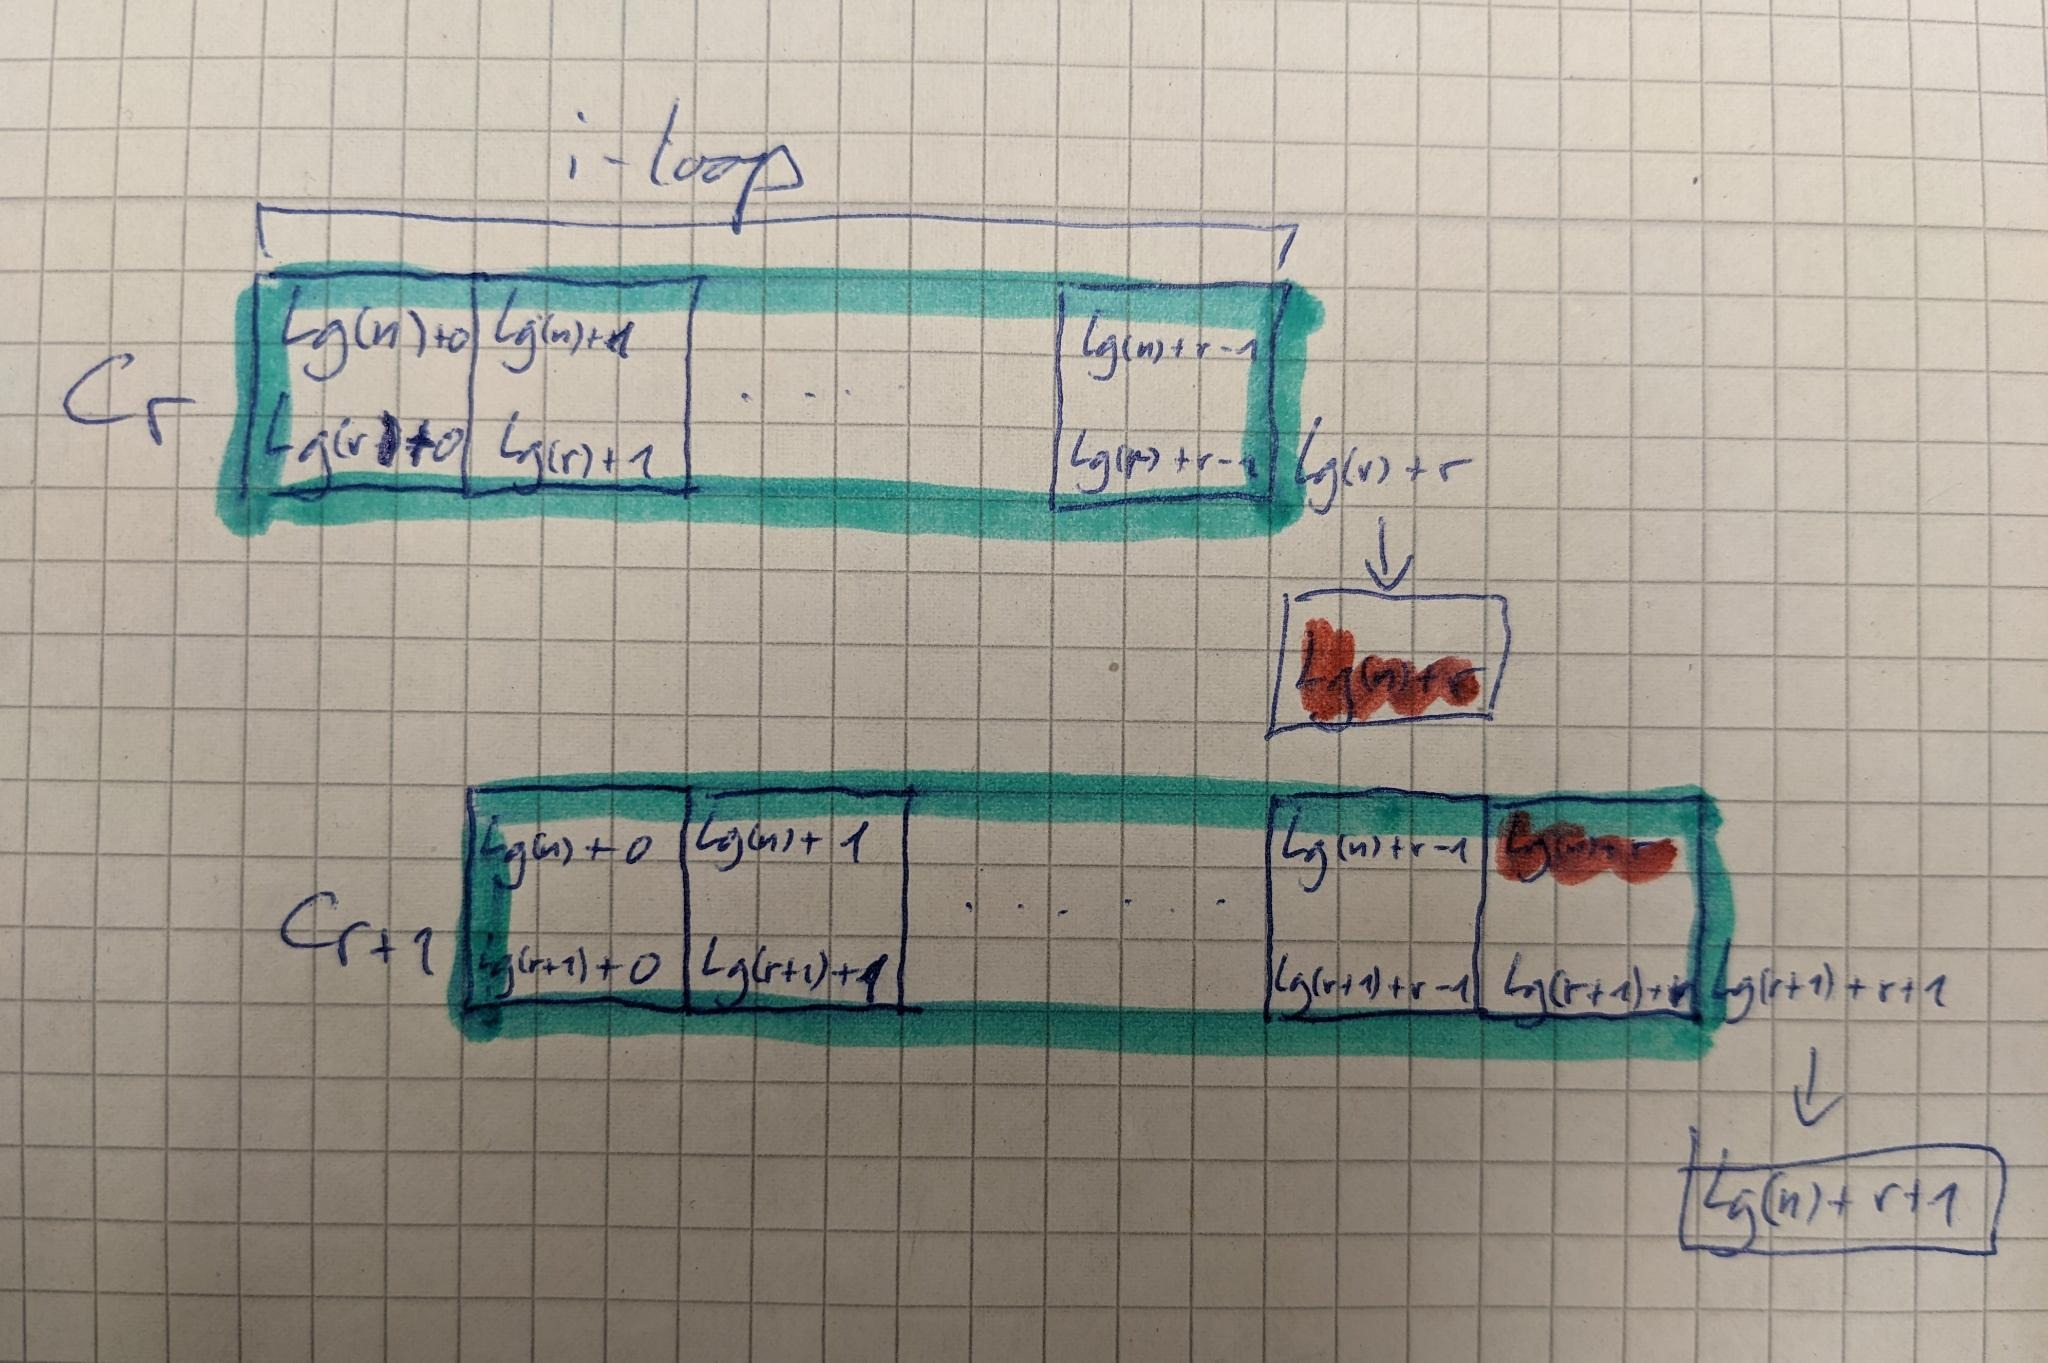
\includegraphics[width=10cm]{images/algo_2_parallel.jpeg}
	\caption{Algorithm~\ref{algo: solve linear equation} parallelization}
 \end{figure}
	\section{GPU Implementation}

\textcite{bellChapter26Thrust2012}, \url{https://nvidia.github.io/thrust/}

or

\url{https://github.com/JuliaGPU/CUDA.jl} (CuArray)


	\printbibliography[heading=bibintoc]	
\end{document}